% --------------------------------------------------------------------------------------------------
% Section: Diagnostic Approaches
% Overview of methods used to detect and evaluate lung cancer
% --------------------------------------------------------------------------------------------------

\section{Diagnostic Approaches}

% --------------------------------------------------------------------------------------------------
% Subsection: Imaging Techniques
% Describes CT, PET, and X-ray uses in lung cancer diagnosis
% --------------------------------------------------------------------------------------------------

\subsection{Imaging Techniques: CT, PET, and X-ray}

% Chest X-ray: initial diagnostic tool
\begin{itemize}
    \item \textbf{Chest X-ray:} Often the first imaging test that primary care providers perform 
    when lung cancer is suspected. Although less detailed than CT or PET, X-rays can provide quick 
    information about the presence of abnormal masses in the lungs. However, small tumors or 
    early-stage lung cancer may not be visible on an X-ray chest scan. \cite{lung_cancer_diagnosis}
\end{itemize}

\vspace{1em}
\begin{center}
    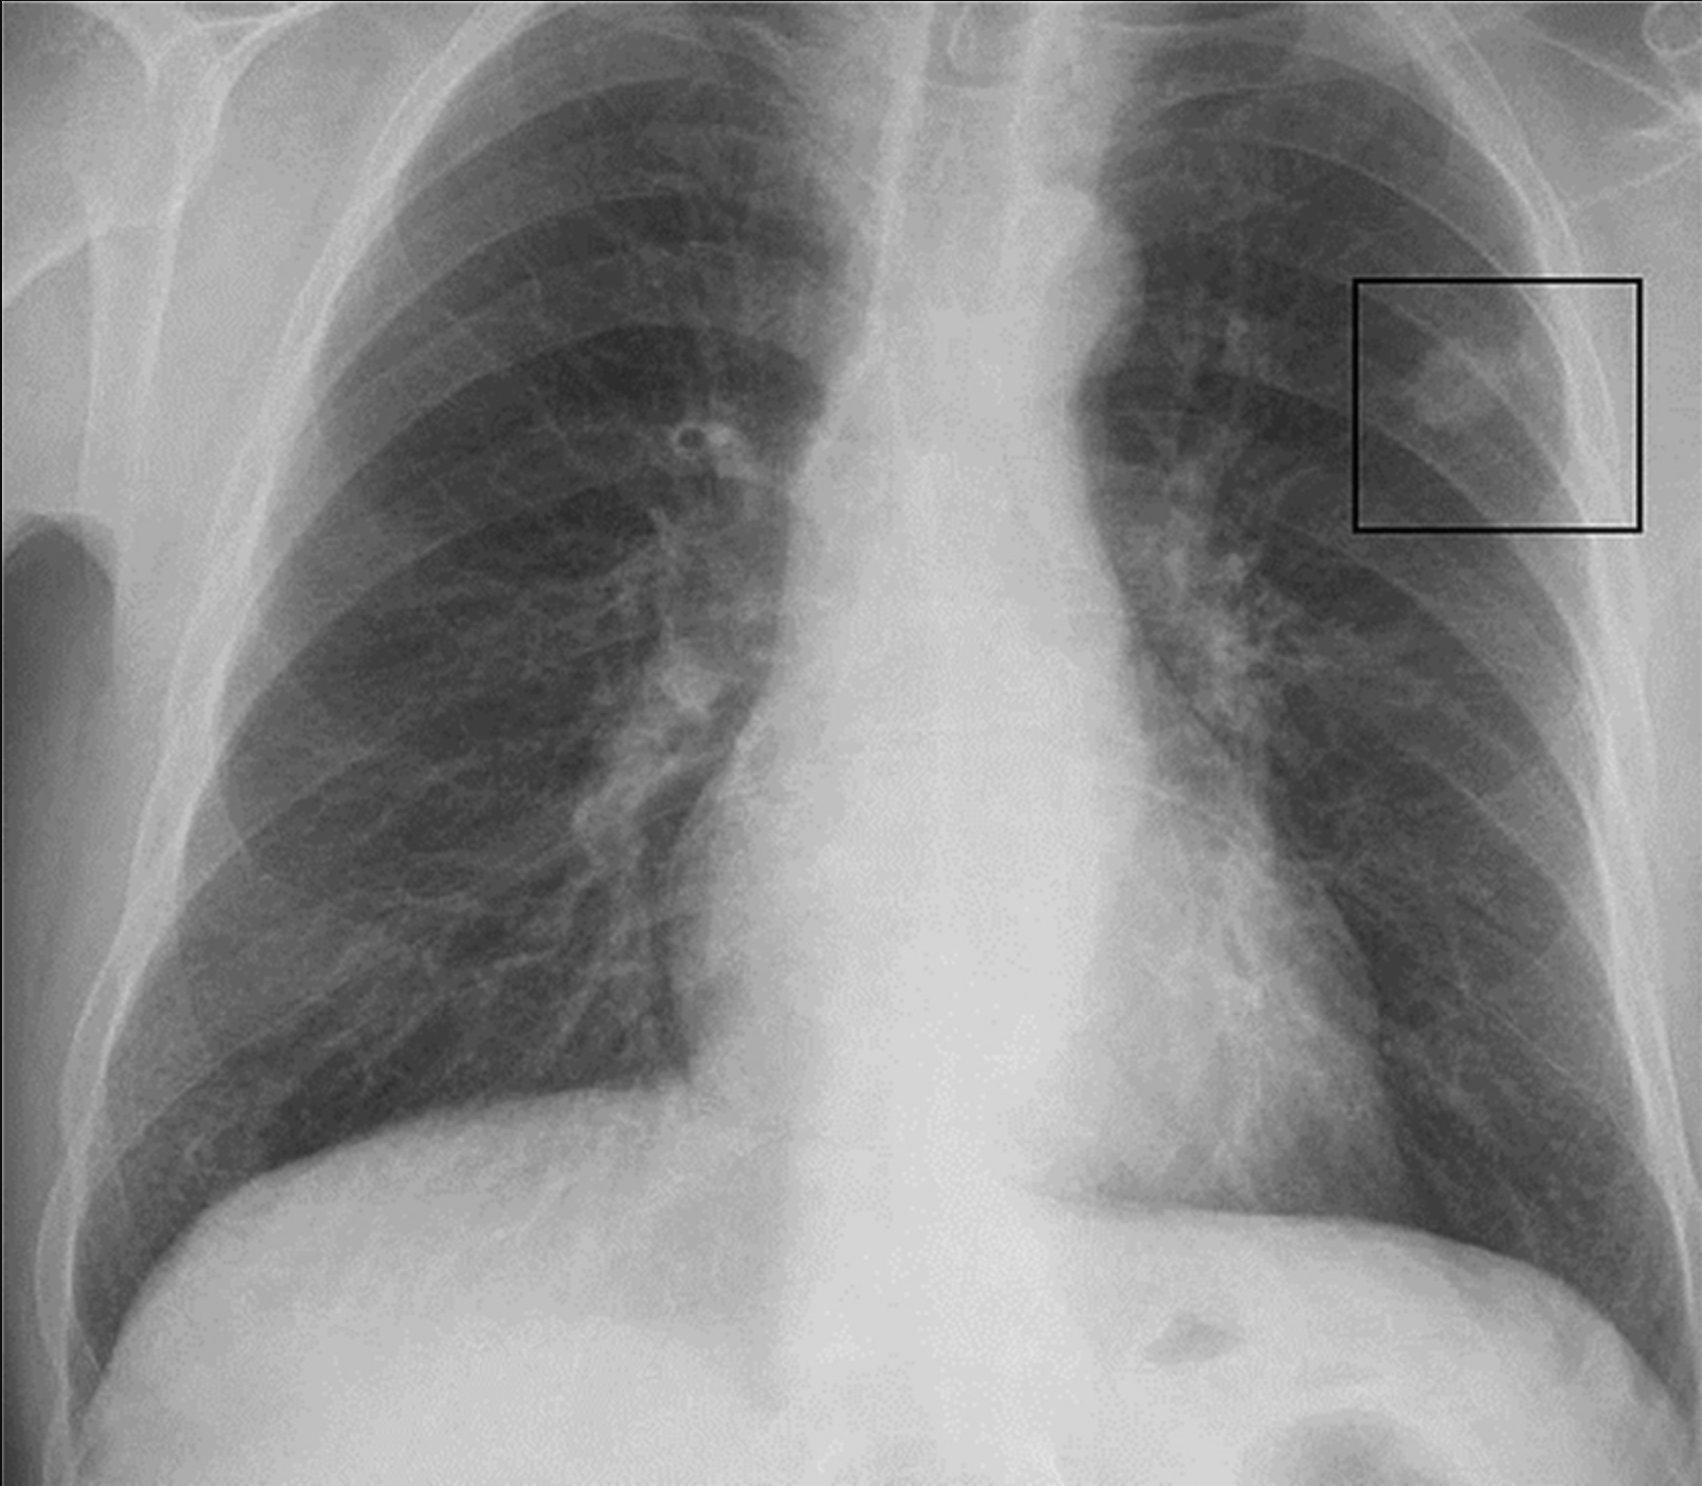
\includegraphics[width=0.5\textwidth]{../assets/04-diagnosis/lc-x-ray.png}
    
    \small\textit{Chest X-ray scan of patient diagnosed with lung cancer. \cite{inbook}}
\end{center}
\vspace{1em}

% CT: detailed cross-sectional view, monitors treatment response
\begin{itemize}
    \item \textbf{Computed Tomography:} Often used to monitor treatment response and check for 
    recurrence. Provides detailed cross-sectional images of the lungs, allowing for the detection of 
    tumors that may not be visible in a standard chest X-ray. They are particularly valuable for 
    assessing the tumor’s size and whether it has spread to nearby lymph nodes or other parts of the 
    body.
\end{itemize}

\vspace{1em}
\begin{center}
    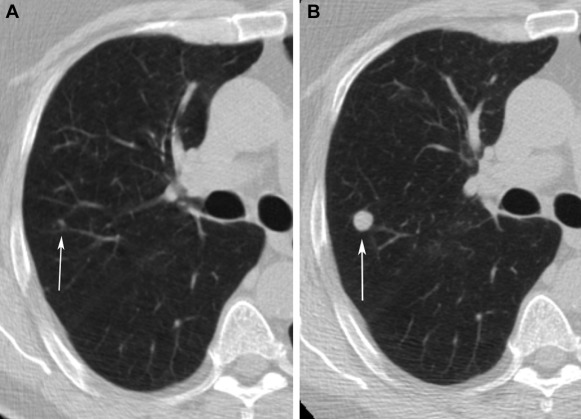
\includegraphics[width=0.75\textwidth]{../assets/04-diagnosis/lc-ct-micronodule-growth.jpg}

    \small\textit{CT scan showing growth of a micronodule (arrows) in the right upper lobe between 
    baseline (A) and 1-year follow-up (B). \cite{MUNDEN20191538}}
\end{center}
\vspace{1em}

% PET: assesses metabolic activity, detects malignancy and spread
\begin{itemize}
    \item \textbf{Positron Emission Tomography:} Employed to assess the metabolic activity of a 
    tumor. Tumors typically exhibit higher metabolic activity than normal tissue, which is 
    visualized as areas of increased uptake of radioactive tracers. PET scans are especially useful 
    in determining the spread of lung cancer and for assessing whether a tumor is benign or 
    malignant.
\end{itemize}

\vspace{1em}
\begin{center}
    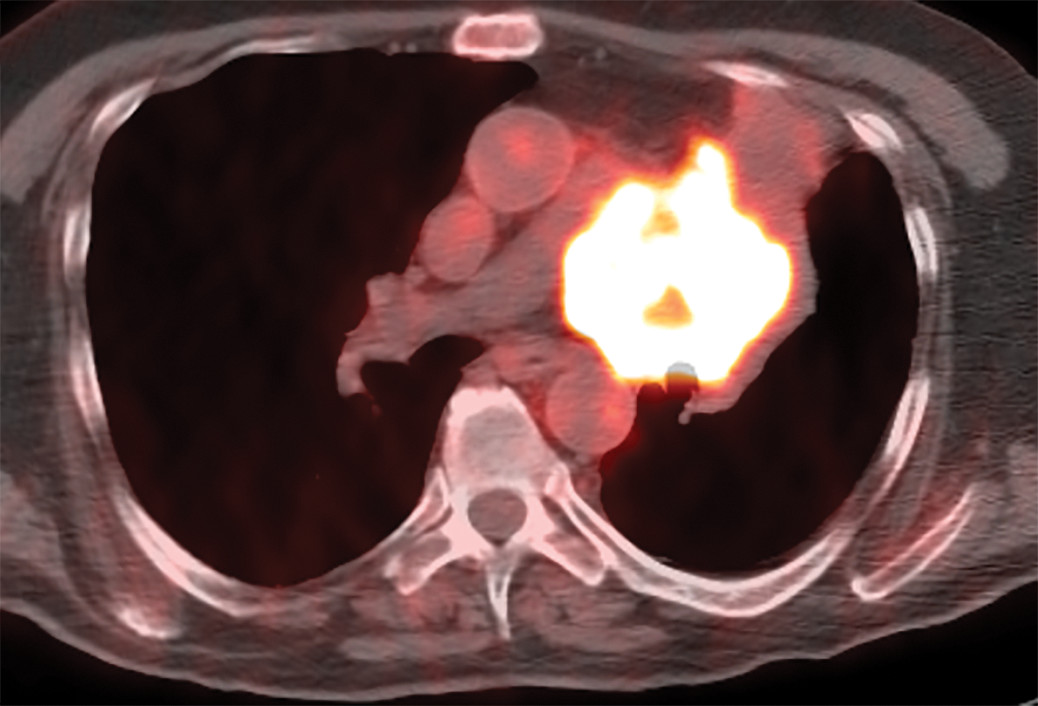
\includegraphics[width=0.75\textwidth]{../assets/04-diagnosis/lc-pet.jpeg}

    \small\textit{PET scan showing growth of a nodule (lighten area). 
    \cite{doi:10.2214/AJR.16.16532}}
\end{center}
\vspace{1em}

% --------------------------------------------------------------------------------------------------
% Subsection: Biopsy and Cytological Analysis
% How tissue samples are collected and analyzed
% --------------------------------------------------------------------------------------------------

\subsection{Biopsy and Cytological Analysis}

% Bronchoscopy: internal airway examination and tissue sampling
\begin{itemize}
    \item \textbf{Bronchoscopy:} A procedure in which a thin, flexible tube is inserted through the 
    mouth or nose into the lungs to collect tissue samples from the airways.
\end{itemize}

\vspace{1em}
\begin{center}
    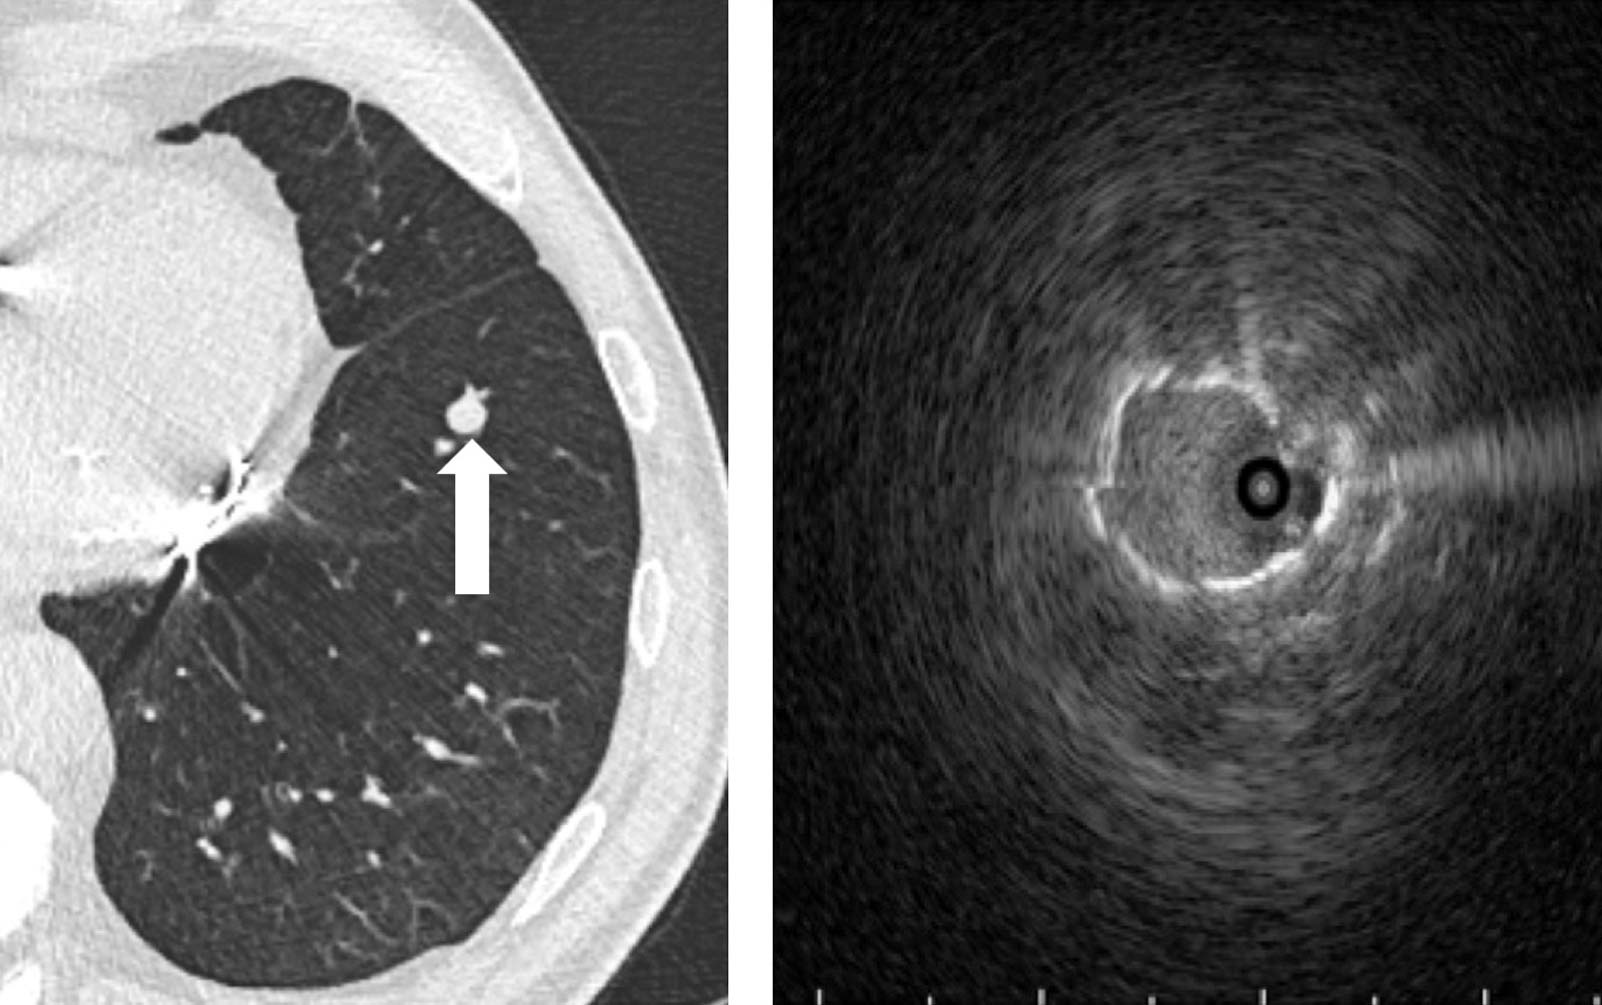
\includegraphics[width=0.65\textwidth]{../assets/04-diagnosis/lc-bronchoscopy.jpg}

    \small\textit{Bronchoscopy lung biopsy in a case of suspected lung cancer. 
    \cite{haas2018bronchoscopic}}
\end{center}
\vspace{1em}

% Needle biopsy: CT- or ultrasound-guided percutaneous tissue sampling
\begin{itemize}
    \item \textbf{Needle Biopsy:} A needle is inserted into the lung to obtain tissue or fluid 
    samples, typically guided by imaging techniques like CT or ultrasound.
\end{itemize}

\vspace{1em}
\begin{center}
    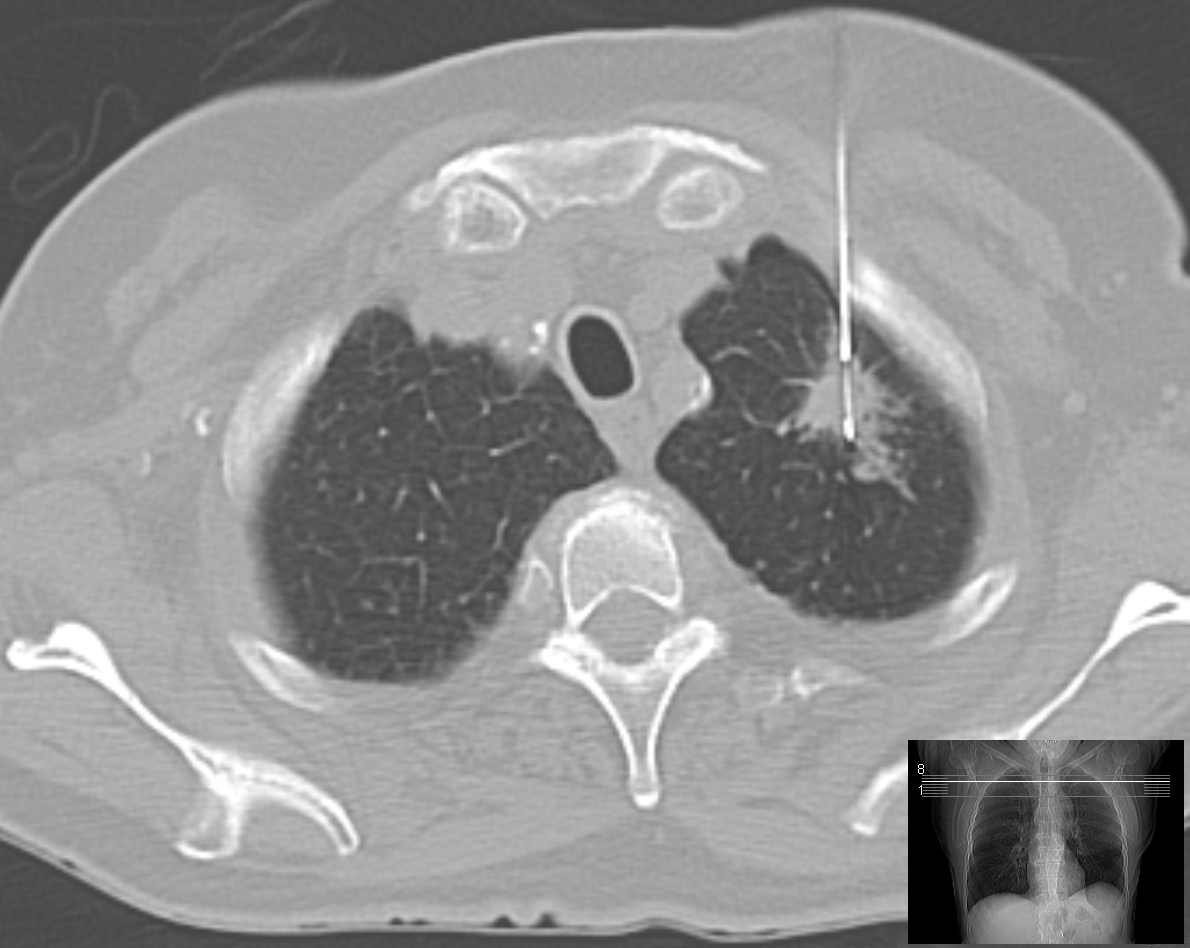
\includegraphics[width=0.60\textwidth]{../assets/04-diagnosis/lc-needle-biopsy.png}

    \small\textit{Percutaneous lung biopsy in a case of suspected lung cancer under control of 
    computed tomography. \cite{enwiki:1188144138}}
\end{center}
\vspace{1em}

\newpage

%Thoracentesis: fluid removal from pleural cavity for analysis
\begin{itemize}
    \item \textbf{Thoracentesis:} This method involves using a needle to remove fluid from the 
    pleural space around the lungs, which can be tested for cancer cells.
\end{itemize}

% Cytology confirms malignancy and may guide treatment options
Once a tissue sample is obtained, it is analyzed through cytological examination. The analysis 
determines the presence of cancerous cells and provides insights into the type of lung cancer. This 
information helps in staging and treatment planning. In some cases, molecular tests are performed to 
identify genetic mutations that may influence treatment choices.

% --------------------------------------------------------------------------------------------------
% Subsection: Tumor Staging and Grading
% Classifies tumor by severity and spread to guide treatment
% --------------------------------------------------------------------------------------------------

\subsection{Tumor Staging and Grading}

% Staging: uses TNM system to describe cancer extent
Staging and grading are essential for determining the prognosis and optimal treatment strategy for 
lung cancer patients. Staging refers to the extent of cancer spread, while grading assesses how 
aggressive the cancer cells are.

\textbf{Staging} is generally performed using the TNM system, which evaluates:

\begin{itemize}
    \item \textbf{T (Tumor):} The size and extent of the primary tumor. For example, T1 indicates a 
    small tumor, while T4 indicates a larger, more invasive tumor.

    \item \textbf{N (Nodes):} Whether cancer has spread to nearby lymph nodes. N0 indicates no lymph 
    node involvement, while N3 indicates extensive nodal spread.

    \item \textbf{M (Metastasis):} Whether the cancer has spread to distant organs. M0 indicates no 
    distant metastasis, while M1 indicates the presence of metastasis.
\end{itemize}

% Grading: evaluates cell abnormality and growth aggressiveness
Together, these three categories allow for the classification of lung cancer into various stages, 
ranging from stage 0 (localized) to stage IV (advanced).

\textbf{Grading} evaluates how abnormal the cancer cells look under a microscope, which helps predict 
how quickly the cancer may grow and spread. The grade ranges from low-grade (well-differentiated) 
to high-grade (poorly differentiated). High-grade tumors tend to grow and spread more aggressively.

% Both staging and grading determine the treatment plan (surgery, chemo, etc.)
Both staging and grading are critical for determining the appropriate treatment approach, whether it 
involves surgery, radiation, chemotherapy, or targeted therapies. Early-stage cancers (stages I and 
II) may be treatable through surgery, while more advanced cancers (stages III and IV) often require 
systemic treatments like chemotherapy and immunotherapy.

% --------------------------------------------------------------------------------------------------
% Subsection: Summary
% Recaps importance of diagnostic methods and early detection
% --------------------------------------------------------------------------------------------------

\newpage

\subsection{Summary and Importance of Diagnostic Approaches}

Accurate and timely diagnosis of lung cancer is essential for selecting the most appropriate 
treatment and improving patient outcomes. Imaging techniques, biopsy and cytological analysis, and 
tumor staging and grading are crucial components in this process. Early detection, particularly in 
high-risk individuals, can significantly improve survival rates and quality of life. Continued 
advancements in diagnostic technology, along with more personalized approaches to treatment, offer 
hope for better management of lung cancer in the future.
